\documentclass[a5paper,10pt]{report}
\usepackage[T1]{fontenc}
\usepackage[utf8]{inputenc}
\usepackage[francais]{babel}
\usepackage{xcolor}
\usepackage[final]{pdfpages}

% % % Personnalisation des couleurs % % %
\definecolor{couleurFonce}{RGB}{0,92,133}
\definecolor{couleurClaire}{RGB}{100,151,186}
\definecolor{couleurTexte}{RGB}{255,255,255}

% % % Personnalisation diverses % % %
\sloppy
\renewcommand{\familydefault}{\sfdefault}

\usepackage{pageDeGarde-livret}

\begin{document}
\pageDeGarde[nomFormation={Formations du département d'informatique},typeDocument={Livret de l'étudiant}, anneeUniversitaire={2012-2013}]

\includepdf[fitpaper,pages=-]{preambule.pdf}
% fitpaper pour inclure le fichier pdf en pleine page (sans marges)
% pages pour sélectionner les pages souhaitées du pdf
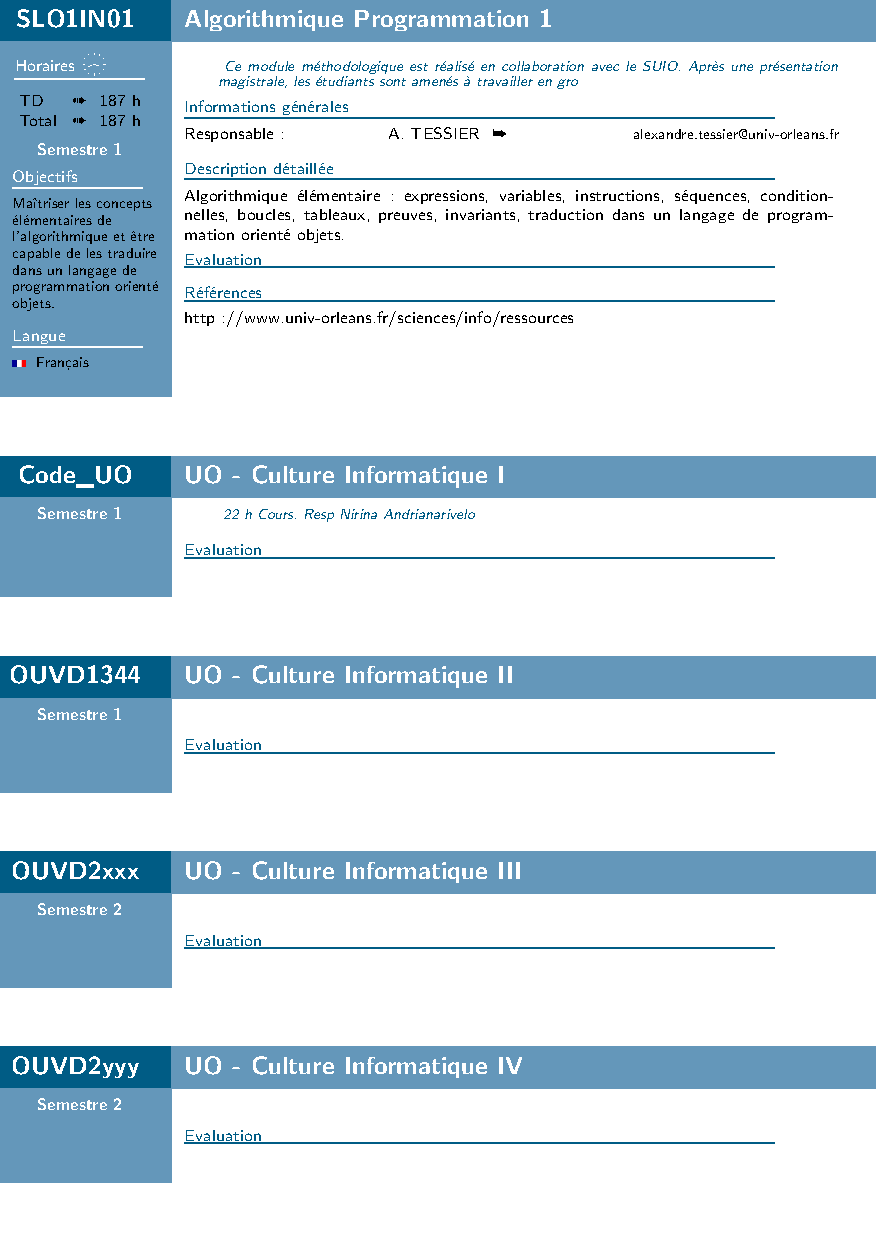
\includepdf[fitpaper,pages=-]{modules.pdf}
\end{document}
